\section{Eksponenttifunktio}

Potenssifunktiossa $f(x) = x^n$ muuttuja $x$ on kantalukuna. Jos muuttuja
$x$ on sen sijaan eksponenttina, saadaan joukko funktioita, joita
kutsutaan \emph{eksponenttifunktioiksi}.

\laatikko{Eksponenttifunktiot ovat muotoa $f(x) = a^x$, $a > 0$,
$a \neq 1$ olevia funktioita.}

Eksponenttifunktioita on kahta tyyppiä: kasvavia ja väheneviä.
Kasvavilla eksponenttifunktioilla $a>1$, esimerkiksi

\begin{center}
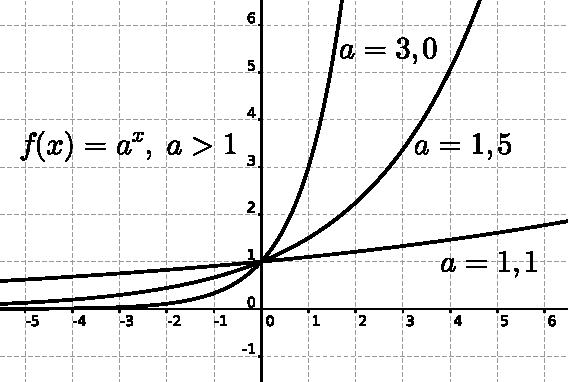
\includegraphics{pictures/apotenssiinxaisompikuinyksi.pdf}
\end{center}

Vähenevillä eksponenttifunktioilla $0<a<1$, esimerkiksi

\begin{center}
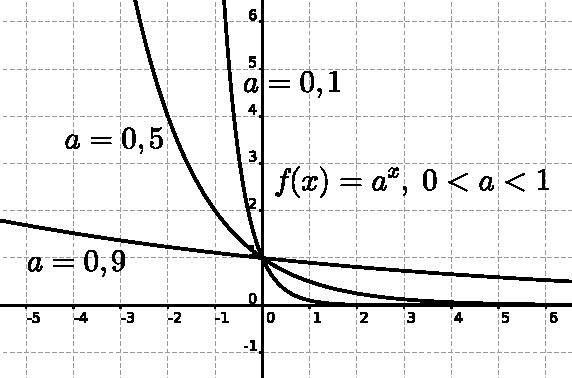
\includegraphics{pictures/apotenssiinxaisompikuinnolla.pdf}
\end{center}

Negatiiviselle kantaluvulle ei ole määritelty yleistä reaalilukupotenssia, 
joten eksponenttifunktiota ei ole määritelty, kun $a < 0$. 

Kun $a=0$ tai $a=1$, eksponenttifunktio pelkistyy vakiofunktioksi.
Lisäksi $0^0$:a ei ole määritelty, joten vaaditaan, että
eksponenttifunktion kantaluvulle $a$ pätee $a>0$ ja $a \neq 1$.

%\emph{Eksponenttiyhtälö} muodostuu, kun kysytään, millä $x$:n arvoilla %eksponenttifunktio saavuttaa tietyn arvon.

\begin{esimerkki}
Millä muuttujan $x$ arvoilla eksponenttifunktio $f(x) = 2^x$ saa arvon
$f(x) = 64$?

\textbf{Ratkaisu.}
Kirjoitetaan tehtävä yhtälöksi: $2^x = 64$. Kokeilemalla huomataan,
että $x = 6$ ratkaisee yhtälön.

Varmistutaan vielä siitä, että yhtälöllä ei ole muita ratkaisuja.
Eksponenttifunktion kantalukuna on $2$, joten eksponenttifunktio on
kasvava. Funktio $f(x) = 2^x$ ei siis voi saada uudelleen arvoa $64$,
kun $x > 6$. Samasta syystä $f(x)$ ei voi olla $64$, kun $x < 6$.

Ainoa ratkaisu yhtälölle on siis $x = 6$.
\end{esimerkki}

\begin{esimerkki}
Millä muuttujan $x$ arvoilla eksponenttifunktio
$f(x) = \left( \frac{1}{2} \right)^{x}$ saa arvon
$f(x) = 1/5$?

\textbf{Ratkaisu.}
Edellisen esimerkin tavoin kokeillaan $x$:n eri arvoja. Havaitaan,
että kun $x = 2$, funktio saa arvon $f(x) = \frac{1}{4}$, ja
kun $x = 3$, on $f(x) = \frac{1}{8}$. Ratkaisu on siis välillä
$2 < x < 3$.

Ratkaisun etsimistä voidaan jatkaa kokeilemalla esimerkiksi
arvoa $x = 2,5$. Näin päästään lähemmäksi ratkaisua, mutta
yhtälön ratkaisu on irrationaalinen, joten sen desimaalikehitelmä
on äärettömän pitkä ja jaksoton. Tarkkaa ratkaisua ei siis saada tällä menetelmällä.

Yleisen eksponenttiyhtälön tarkkaan ratkaisemiseen palataan myöhemmillä
matematiikan kursseilla.
\end{esimerkki}


\subsection*{Eksponentiaalinen malli}

Kun eksponenttifunktiota käytetään kuvaamaan jotakin reaalimaailman
ilmiötä, siitä käytetään nimeä \emph{eksponentiaalinen malli}.

Eksponentiaalinen malli on eräs yleisimmin käytetyistä matemaattisista
malleista. Sillä kuvataan sellaista kasvua tai vähenemistä, jossa
kullakin ajanhetkellä funktion hetkellinen muutos on suoraan
verrannollinen funktion sen hetkiseen arvoon. Tämä muotoillaan
täsmällisesti myöhemmillä matematiikan kursseilla.

\begin{esimerkki}
Soluviljelmässä olevien \emph{Escherichia coli} -bakteerien
määrää voidaan kuvata eksponentiaalisella mallilla: ajanhetkellä
$t = 0$ bakteerien lukumäärä on $1$, ja kullakin aika-askeleella
bakteerien lukumäärä tuplaantuu. Malli voidaan kirjoittaa
\[
f(t) = 2^t, t \ge 0,
\]
jossa $f(t)$ on bakteerien lukumäärä ajanhetkellä $t$.
% vanha sivulaatikko
\laatikko{
Huomaa, että esimerkissä funktion $f(t)$ arvot voivat
olla myös rationaalisia tai irrationaalisia, vaikka bakteerien
määrä on kokonaisluku. Yleensä tätä ei pidetä ongelmallisena,
vaan funktiota voidaan käsitellä, ikään kuin bakteerien määrä
olisi jatkuvasti kasvava suure.
}
\end{esimerkki}

\begin{esimerkki}
Radioaktiivisessa hajoamisessa atomiydinten lukumäärää kuvataan
eksponentiaalisella mallilla. Jos ydinten määrä ajanhetkellä
$t = 0$ on $f(t) = k$, malli voidaan kirjoittaa
\[
f(t) = k \cdot \left( \frac{1}{2} \right)^t, t \ge 0,
\]
jossa $f(t)$ on atomiydinten lukumäärä ajanhetkellä $t$. Atomiydinten
lukumäärä siis puolittuu kullakin aika-askeleella.
\end{esimerkki}

\subsection*{Tehtäviä}

\paragraph*{Opi perusteet}

\begin{tehtava}
Olkoon $f(x) = 4^x$. Laske
\begin{enumerate}[a)]
\item $f(0)$
\item $f(3)$
\item $f(\frac{1}{2})$
\end{enumerate}
\begin{vastaus}
\begin{enumerate}[a)]
\item $1$
\item $64$
\item $2$
\end{enumerate}
\end{vastaus}
\end{tehtava}

\begin{tehtava}
Olkoon $f(x) = 10^x$. Millä $x$:n arvoilla
\begin{enumerate}[a)]
\item $f(x) = 1000$
\item $f(x) = \frac{1}{100}$
\item $f(x) = -1$?
\end{enumerate}
\begin{vastaus}
\begin{enumerate}[a)]
\item $3$
\item $6$
\item Ei ratkaisua.
\end{enumerate}
\end{vastaus}
\end{tehtava}

\paragraph*{Hallitse kokonaisuus}
\begin{tehtava}
Minkä kahden kokonaisluvun välissä yhtälön
$10^x = 500$ ratkaisu on?
\begin{vastaus}
Ratkaisu on lukujen $2$ ja $3$ välissä.
\end{vastaus}
\end{tehtava}


\begin{tehtava}
Olkoon $f(t) = 20 \cdot 2^t$ bakteerien lukumäärä soluviljelmässä
ajanhetkellä $t$. Millä ajanhetkellä bakteerien lukumäärä on tasan 160?
\begin{vastaus}
Ajanhetkellä $t = 3$.
\end{vastaus}
\end{tehtava}

\begin{tehtava}
Miten muokkaisit edellisen tehtävän funktiota, jos bakteerien lukumääräksi
halutaan 5 ajanhetkellä $t = 0$?
\begin{vastaus}
$f(t) = 5 \cdot 2^t$
\end{vastaus}
\end{tehtava}

\begin{tehtava}
Millä ajanhetkellä atomiydinten määrä on alle $1/200$ alkuperäisestä?
\begin{vastaus}
Ajanhetkellä $t = 8$.
\end{vastaus}
\end{tehtava}

\paragraph*{Sekalaisia tehtäviä}

\begin{tehtava}
(YO 1877 4) Vuosikymmenen 1860--70 kuluessa lisääntyi Helsingin väkiluku puolella vuoden 1860 väkiluvulla. Jos väkiluvun lisäys tapahtuisi seuraavinakin vuosikymmeninä samassa suhteessa, paljonko väkeä Helsingissä olisi 1890, kun siellä 1860 oli 21~700 asukasta? 
	\begin{vastaus}
	73~200 (pyöristämättä 73~237,5)
	\end{vastaus}
\end{tehtava}


% % tähän parempi tehtävä atomiytimistä
%\begin{tehtava}
%Millä ajanhetkellä atomiydinten määrä on alle $1/200$ alkuperäisestä?
%\begin{vastaus}
%Ajanhetkellä $t = 8$.
%\end{vastaus}
%\end{tehtava}
